\chapter{O que é o \textrm{\LaTeX}?}
\label{cap:latex}

\lettrine[lines=3]{\color{azulUFRB} \initial R}{esumidamente}, o \hologo{LaTeX} 
é um \textsf{sistema} de preparação de documentos para composição tipográfica 
de alta qualidade. 
Mas\ldots\ o que isso realmente siginifica?  

\section{Arte e Tecnologia juntos} %--------------------------------------

Quando penso numa definição sobre \latex\ geralmente associo a uma função de 
várias variáveis (sou matemático, o que posso fazer? \emoji{grin}). 
E, duas dessas variáveis são fundamentais: \textit{engine} e \textit{format}.
O termo \textit{engine} pode ser traduzido de diversas formas, mas entendo como 
\textsf{mecanismo} ou \textsf{motor}; da mesma forma, o termo \textit{format}, 
pode significar \textsf{formato} ou \textsf{linguagem}. 
Tais conjuntos de ferramentas, são usadas para produzir um arquivo final de alta 
qualidade tipográfica (hoje, geralmente, com extensão \texttt{.pdf}). 
Então, ao usarmos o \latex, escrevemos um \textsf{manuscrito} que mistura texto 
com códigos; e, depois de um processo de \textsf{composição} (que, geralmente 
falamos \textsf{compilação}, por conta de aspectos ligados à computação) é gerado, 
dentre outras coisas, um arquivo final com qualidade já de impressão. 

Falando nisso \ldots\ você ainda lembra o que é um \textsf{manuscrito} e do 
processo que era produzir um texto com qualidade suficiente para imperssão? 
Na época em que se usava papel e caneta, um professor de matemática, por exemplo, 
escrevia suas notas de aulas e as usava até o papel ficar amarelado. 
Eventualmente, um colega descobre essas notas e as usa quando ministra a mesma 
disciplina, posteriormente. 
Então, afirma que essas preciosas notas deveriam ser publicadas. 
Convencido, o professor que as escreveu procura uma editora e apresenta o 
manuscrito (que possivelmente passou por um processador de texto padrão). 
A editora, então, escolhe as fontes para o texto e símbolos matemáticos; o 
espaçamento adequado; qual tamanho de papel; como será a disposição do texto 
nesta folha; passa por outro programa que melhora o texto digitado no 
processador de texto padrão; etc.; para depois enviar para impressão. 
Todo esse processo é o que se chama de \textsf{composição tipográfica}.

\begin{center}
  \begin{PostItNote}[Render=tikz, Color=douradoUFRB]
    \sffamily
    Podemos afirmar, portanto, que o \latex\ é um conjunto (sistema) estruturado 
    de ferramentas que envolve um \textbs{formato} de escrita específico e uso 
    de um \textbs{mecanismo} para \textbs{compor tipograficamente} um manuscrito 
    com qualidade profissional. 
  \end{PostItNote}
\end{center}

Apenas por curiosidade, a Figura~\ref{fig:phd} mostra como era comum, numa época 
anterior ao \latex\ ou a sistemas tipográficos eletrônicos rudimentares, escrever 
(literalmente) \textsf{à mão}, as equações com simbologias específicas. 

\begin{figure}[!htbp]
  \centering
  \caption{Página 33 da tese de doutorado de Richard Feynman}
  \label{fig:phd}
  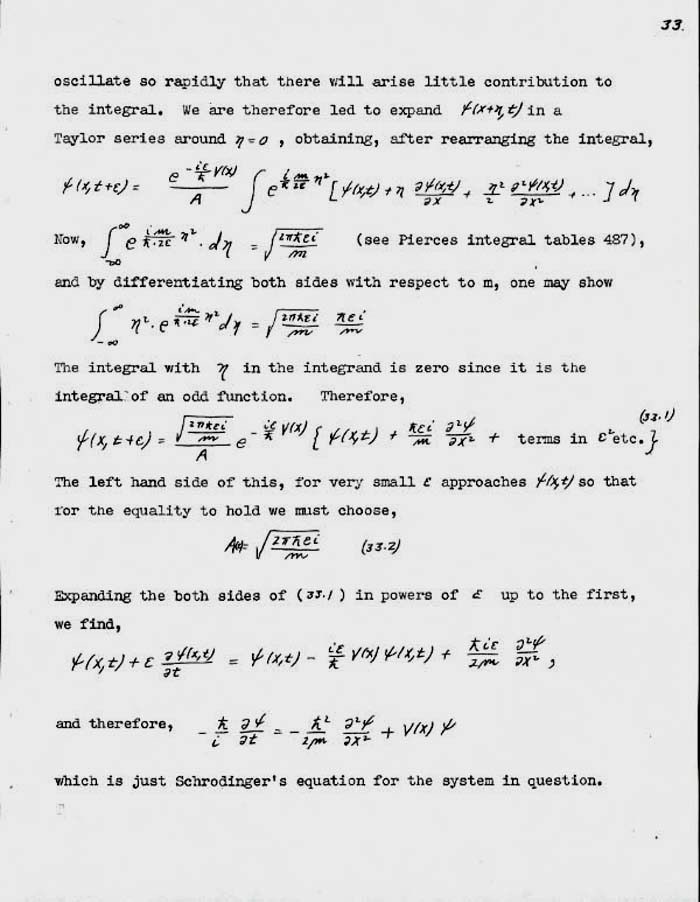
\includegraphics[width = \textwidth]{phd33} \\
  {
  \small \sffamily
  \textsf{Fonte:} \href{https://ysfine.com/feynman/fthesis.html}{https://ysfine.com/feynman/fthesis.html}
}
\end{figure}

O nome \latex\ é uma junção de dois outros: \hologo{La} + \TeX. 
O primeiro, veio de \texttt{\textbf{La}}mport, que é o sobrenome do matemático e 
cientista da computação  estadunidense chamado \textsf{Leslie B. Lamport}, que 
na década de 80 criou um conjunto bem estruturado de \textsf{macros} (a grosso 
modo, pense num conjunto de mapeamentos/atalhos de outros comandos mais básicos, 
denominados \textsf{primitivos}) para uma linguagem de programação exclusivamente 
voltada à composição tipográfica: o \TeX. 
Portanto, o \latex\ é uma linguagem de \textsf{marcação} pra uma linguagem de 
\textsf{programação} denominada \TeX. 
O nome \TeX\ é uma junção de três letras gregas: $\tau$ (\textsf{tau}), 
$\varepsilon$ (\textsf{epsilon}) e $\chi$ (\textsf{chi}) --- esta última, lê-se 
``ki''; e possui a mesma raíz etimológica das palavras \textsf{arte} ({\grega τέχνη}) 
e \textsf{tecnologia} ({\grega τεχνολογία}). 
Ou seja, o autor dessa linguagem de programação, propositalmente, escolheu uma 
palavra que expressasse uma ideia de beleza (tal como a arte da {\caligra \Large Caligrafia})
e tecnologia (pois usou e usa os mais sofisticados algorítimos para composição 
tipográfica).
O leve deslocamento para baixo da letra \texttt{E}, foi para deixar claro que 
trata-se de composição tipográfica. 

A história do \latex\ é indissasociável do \TeX. 
E, a história deste último é bem peculiar: \textsf{Donald Ervin Knuth}, no final 
da década de 1970, recebeu as primeiras amostras de seu próprio livro de 
computação, \textit{The Art of Computer Programming}, produzido por um novo 
sistema tipográfico de sua editora. 
O resultado não agradou ao Knuth que, como cientista da computação, compreendeu 
que a disposição tipográfica de um texto é, em essência, um processo estruturado 
e lógico de preenchimento ou não de tinta no papel. 
E, isso poderia ser traduzido em linguagem computacional: 0 (sem tinta) ou 1 (com tinta). 
Em resumo: criou uma linguagem de programação voltada à composição tipográfica, 
que viria revolucionar a escrita de textos impressos, em especial os textos que 
envolviam Matemática (mas, não exclusivamente ela), porque não encontrou beleza 
no resultado tipográfico de um de seus livros. \emoji{joy}\emoji{upside-down-face}
O próprio Knuth criou um conjunto de macros para o \TeX, denominado \textit{Plain \TeX}, 
para que pudesse usar alguns conjuntos de comandos que frequentemente precisava. 
Mas, Lamport estruturou os conjuntos de macros de maneira tão organizada e eficiente 
que logo se popularizou entre os matemáticos (ou quem precisava escrever algo que 
envolvesse principalmente expressões matemáticas). 
Você pode ler mais sobre a história do \TeX\ neste \textit{link}: 
\linkExt{https://tug.org/whatis.html}{History of TeX}. 

Entretanto, ainda havia limitações em muitos aspectos no \latex: tanto no 
conjunto de macros, quanto nos mecanismos associados à composição tipográfica. 
Outras versões foram surgindo e essas limitações sendo sanadas. 
A última versão modificada pelo próprio Lamport foi a \hologo{LaTeX}~$2.09$. 
Depois disso o projeto passou para um grupo de desenvolvedores que trouxeram 
significativas mudanças estruturais, mas sempre com o princípio de manter a 
compatibilidade naquilo que era possível das versões anteriores. 
Assim, em 1994, surge o \hologo{LaTeX2e} (o $\varepsilon$, provavelmente aparece aí 
para passar a ideia de que a modificação foi mínima/pequena --- fazendo uma 
alusão a ideia do $\varepsilon$ na definição de limites, em Matemática)
\footnote{ 
  $ \lim\limits_{x \to a} f(x) = L$ se para todo $ \varepsilon > 0 $ dado, existir 
  $ \delta > 0 $, tal que a seguinte afirmação é verdadeira:
  \[
    \vert x - a \vert < \delta \Rightarrow \vert f(x) - L \vert < \varepsilon,
  \]
  ou seja, $L$ é o \textsf{limite} de $f(x)$ quando $x$ tende ao real $a$, se a 
  distância de $ f(x) $ ao número real $ L $ é ``tão pequena quanto se queira'', 
  desde que $ x $ esteja ``suficientemente próximo'' de $a$.
} que continua sendo a versão atual (\the\year). 
Havia uma possibilidade de uma nova reestruturação, agora mais significativa, no 
\hologo{LaTeX2e}, passando para uma versão denominada \latex$3$. 
Entretanto, por conta do princípio da compatibilidade para versões anteriores, 
essa ideia foi abandonada e decidiu-se modernizar gradualmente o \hologo{LaTeX2e}. 
Você pode saber mais sobre o \LaTeX 3 e seus desdobramentos atuais no \textit{link}:
\linkExt{https://www.latex-project.org/latex3/}{The \LaTeX\ Project}.

\begin{center}
  \begin{PostItNote}[Render=tikz, Color=douradoUFRB]
    \sffamily
    Note que, atualmente, quando falamos ``\latex'', estamos implicitamente 
    falando da versão \textrm{\hologo{LaTeX2e}}; mas, por simplicidade, usaremos 
    apenas a primeira notação.
  \end{PostItNote}
\end{center}

\section{Mais sobre os mecanismos de composição tipográfica}

A modernização sempre acompanhou o \latex. 
A saída final de um documento, no início do \latex, era em \texttt{DVI} 
(\textit{device independent file format}).  
O \texttt{PDF} foi criado apenas em 1992 e, com sua popularidade, o mecanismo 
de composição do \latex\ foi modificado. 
Inicialmente, havia um conversor do \texttt{DVI} para \texttt{PDF}; depois, em 
1999, surgiu o \hologo{pdfTeX} que produzia o \texttt{PDF} final diretamte, além 
de muitas outras funcionalidades: melhora na quebra de parágrafos; melhora 
significativa no processo de deixar o texto ``justificado''; etc. 


\begin{center}
  \begin{PostItNote}[Render=tikz, Color=douradoUFRB]
    \sffamily
    Como pronunciamos a palavra \latex ?
    Existem duas formas aceitáveis: ou {\tt La-Téc}, ou {\tt Lei-Téc}. 

    Evite falar {\tt La-Técks}, ou pior {\tt Lá-Tecks} (que é aquela seiva 
    branca encontrada em algumas árvores). 
    Além disso, escreva LaTeX, quando não puder escrever \latex 
    --- evite Latex.
  \end{PostItNote}
\end{center}

\begin{figure}[!htbp]
  \centering
    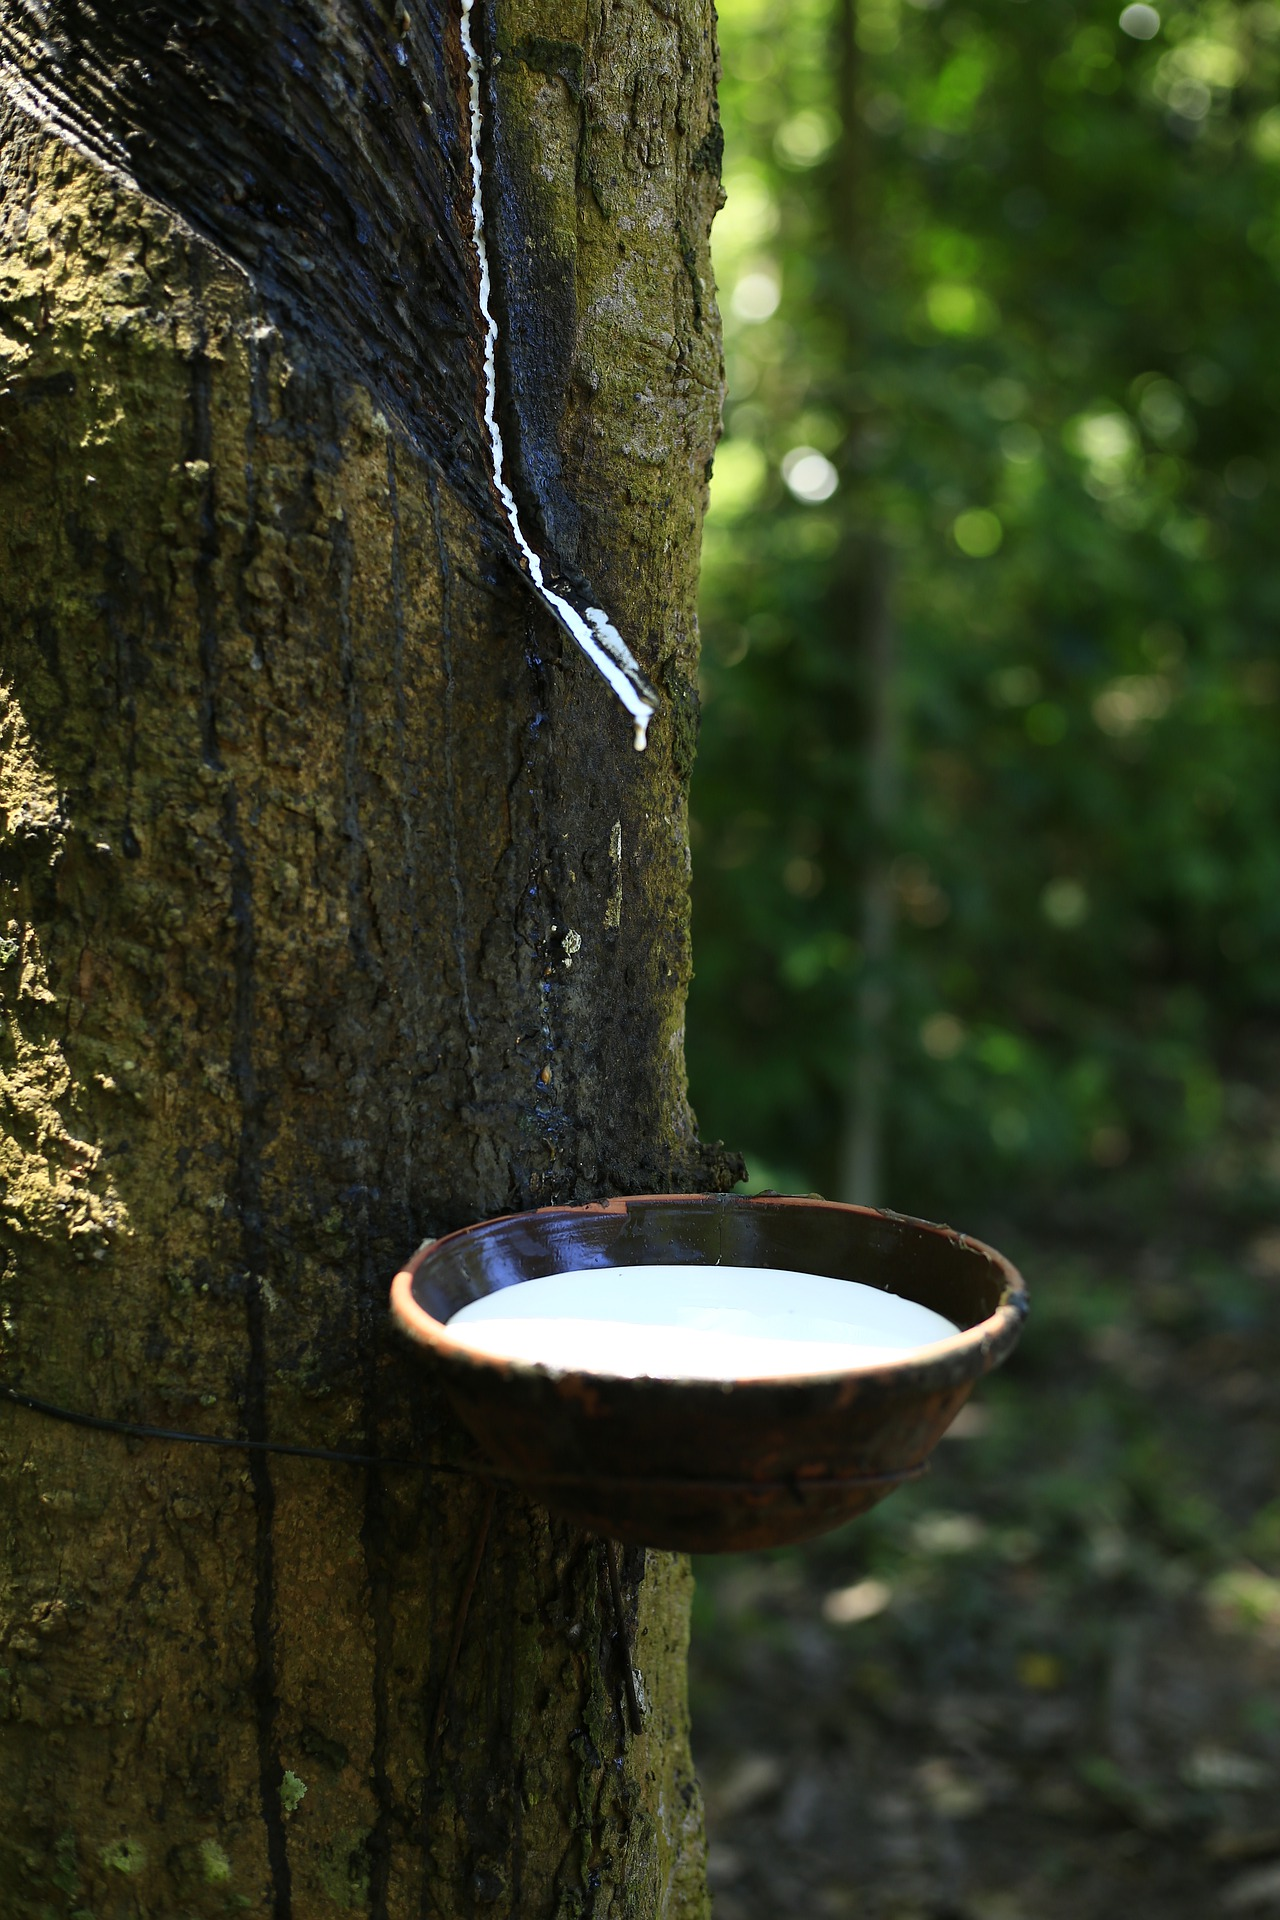
\includegraphics[width=0.4\textwidth]{seringueira}
  \caption{Isso é Látex, não \textrm{\hologo{LaTeX}}}
\end{figure}
